\documentclass[hidelinks]{ctexart}

\usepackage[sensei=陈向军/刘明辉,gakka=原子物理学,section=Tadenshi,gakkabbr=AP]{styles/kurisu}

\usepackage{van-de-la-illinoise}

\begin{document}

\section{多电子原子} % (fold)
\label{sec:多电子原子}

\subsection{氦原子的光谱与能级} % (fold)
\label{sub:氦原子的光谱与能级}

\begin{figure}[ht]
    \centering
    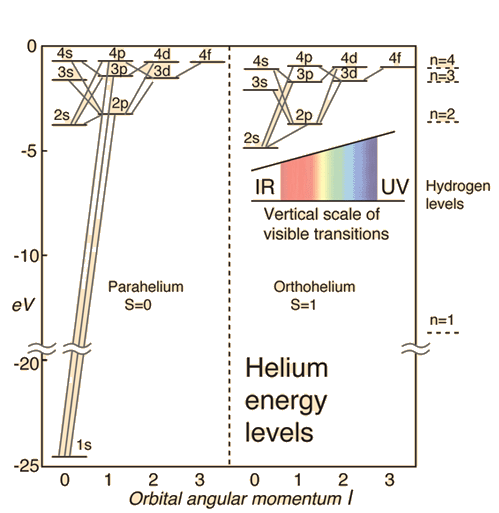
\includegraphics[width=9cm]{src/heliumlev.png}
\end{figure}

\newpoint{}氦原子的光谱有两套谱线系, 即两个主线系, 两个漫线系, 两个锐线系. 两套谱线的结构有显著差别, 其中一套简单(仲氦)而另一套复杂(正氦).
\newpoint{}一套能级是单重结构, 另一套是三重结构.
\newpoint{}三重态能级低于单重态能级, $\ce{2 ^3S_{1}}$的能级比$\ce{2 ^1S_{0}}$的能量低$\SI{0.786}{\eV}$.
\newpoint{}$n=1$的原子不存在三重态.
\newpoint{}$\ce{2 ^3S_1}$和$\ce{2 ^1S_0}$的寿命都很长, 称为亚稳态. 例如$\ce{2 ^1S_0}$的寿命为$\SI{19.5}{\milli\second}$.
\newpoint{}基态和第一激发态之间有很大的能量差, $\SI{19.819}{\eV}$. 氦的电离能是所有元素中最大的, 为$\SI{24.587}{\eV}$.

% subsection 氦原子的光谱与能级 (end)

\subsection{Pauli不相容原理} % (fold)
\label{sub:pauli不相容原理}

\subsubsection{全同粒子} % (fold)
\label{ssub:全同粒子}

\newpoint{}所有内禀属性皆相同的粒子谓全同粒子.
\newpoint{}在波函数重叠的区域, 本质上无法区分两个粒子.
\newpoint{全同性原理} 全同粒子组成的体系中, 交换任意两个粒子不会引起物理状态的变化.

% subsubsection 全同粒子 (end)

\subsubsection{波函数的交换对称性} % (fold)
\label{ssub:波函数的交换对称性}

将两个电子的全部坐标(空间和自旋)分别记为$q_1$和$q_2$, 引入交换算符$P_{12}$如
\[ P_{12}\psi\pare{q_1,q_2} = \psi\pare{q_2,q_1}. \]
按照全同性原理, 交换两个粒子不改变体系的物理状态, 故
\[ P_{12}\psi\pare{q_1,q_2} = \lambda\psi\pare{q_2,q_1}. \]
从而
\[ P^2_{12}\psi\pare{q_1,q_2} = \lambda^2\psi\pare{q_1,q_2} = \psi\pare{q_1,q_2}. \]
因此$\lambda = \pm 1$.
\begin{cenum}
    \item $\lambda=1$的态满足$P_{12}\psi\pare{q_1,q_2} = \psi\pare{q_1,q_2}$, 谓交换对称的.
    \item $\lambda=-1$的态满足$P_{12}\psi\pare{q_1,q_2} = -\psi\pare{q_1,q_2}$, 谓交换反对称的.
\end{cenum}
Boson具有交换对称性, Fermion具有交换反对称性.
\par
对于由全同Fermion组成的系统,
\[ \hat H\psi \pare{q_1,q_2} = E\psi\pare{q_1,q_2}. \]
忽略粒子间的相互作用,
\[ \hat H = \hat H_0\pare{q_1} + \hat H_0\pare{q_2}. \]
波函数可以分离变量,
\[ \psi\pare{q_1,q_2} = \psi\pare{q_1}\psi\pare{q_2}. \]
故可分解为两个粒子各自的Schr\"odinger方程
\[ \begin{cases}
    \hat H_0\pare{q_1} \psi\pare{q_1} = E_1\psi\pare{q_1}, \\
    \hat H_0\pare{q_2} \psi\pare{q_2} = E_2\psi\pare{q_2}.
\end{cases} \]
两个Hamiltonian的形式相同, 有一套能量本征值的本征函数. 设体系的两个粒子中一个处于$\alpha$态, 一个处于$\beta$态, 则体系可能的状态波函数为
\[ \begin{cases}
    \psi = \psi_\alpha\pare{q_1} \psi_\beta\pare{q_2}, \\
    \psi = \psi_\alpha\pare{q_2} \psi_\beta\pare{q_1}.
\end{cases} \]
两个态不满足交换对称/反对称性. 构造新的波函数
\[ \begin{cases}
    \displaystyle \psi\+_S_\pare{q_1,q_2} = \rec{\sqrt{2}} \brac{\psi_\alpha\pare{q_1}\psi_\beta\pare{q_2} + \psi_\beta\pare{q_1}\psi_\alpha\pare{q_2}}, \\
\displaystyle \psi\+_A_\pare{q_1,q_2} = \rec{\sqrt{2}} \brac{\psi_\alpha\pare{q_1}\psi_\beta\pare{q_2} - \psi_\beta\pare{q_1}\psi_\alpha\pare{q_2}}. \\
\end{cases} \]
\newpoint{Pauli不相容原理} 多电子原子中, 不能有两个原子处于完全相同的状态. 即原子中不能有任何两个电子具有完全相同的四个量子数$\pare{n,l,m_l,m_s}$.
\newpoint{}因此两个Fermion, 例如电子, 不能处于相同的状态. 否则
\[ \psi\+_A_\pare{q_1,q_2} = \rec{\sqrt{2}} \brac{\psi_\alpha\pare{q_1}\psi_\alpha\pare{q_2} - \psi_\alpha\pare{q_1}\psi_\alpha\pare{q_2}} = 0. \]

% subsubsection 波函数的交换对称性 (end)

\subsubsection{两个电子的自旋波函数} % (fold)
\label{ssub:两个电子的自旋波函数}

将自旋波函数分解为空间波函数$u$和自旋波函数$\chi\pare{\+vs_1,\+vs_2}$,
\[ \psi\pare{q_1,q_2} = u\pare{\+vr_1,\+vr_2} \chi\pare{\+vs_1,\+vs_2}. \]
对于自旋波函数部分, 单个粒子的自旋状态有$s=1/2$, $m_s = \pm 1/2$. 用$\sigma^+$和$\sigma^-$表示两个自旋, 引入总的自旋角动量$\+vS$满足
\[ \+vS^2 = S\pare{S+1}\hbar^2,\quad S_z = M\+_S_\hbar, \]
总自旋角动量是两个电子自旋的矢量和,
\[ \+vS = \+vs_1 + \+vs_2. \]
单电子的自旋量子数
\[ s_1 = s_1 = \half, \]
故
\[ S = 0,1. \]
当$S = 0$, 有$M\+_S_ = 0$. 当$S = 1$, 有$M\+_S_ = -1,0,+1$. 两个电子的状态有组合
\[ \begin{cases}
    \chi_1 = \sigma_+\pare{1}\sigma_+\pare{2},\\
    \chi_2 = \sigma_+\pare{1}\sigma_-\pare{2},\\
    \chi_3 = \sigma_-\pare{1}\sigma_+\pare{2},\\
    \chi_4 = \sigma_-\pare{1}\sigma_-\pare{2}.
\end{cases} \]
$\chi_1$和$\chi_4$满足交换对称性, 而$\chi_2$和$\chi_3$不满足. 重新构造
\[ \begin{cases}
    \displaystyle \chi\+_S_ = \rec{\sqrt{2}} \brac{\sigma_+\pare{1}\sigma_-\pare{2} + \sigma_-\pare{1}\sigma_+\pare{2}}, \\
    \displaystyle \chi\+_A_ = \rec{\sqrt{2}} \brac{\sigma_+\pare{1}\sigma_-\pare{2} - \sigma_-\pare{1}\sigma_+\pare{2}}.
\end{cases} \]
可以得到交换对称的态(三种情况下电子自旋都有平行部分)
\[ \resumath{\chi\+_S_ = \begin{cases}
    \sigma_+\pare{1}\sigma_+\pare{2}, & M\+_S_ = +1, \\
    \displaystyle \rec{\sqrt{2}} \brac{\sigma_+\pare{1}\sigma_-\pare{2} + \sigma_-\pare{1}\sigma_+\pare{2}}, & M\+_S_ = 0, \\
    \sigma_-\pare{1}\sigma_-\pare{2}, & M\+_S_ = -1,
\end{cases}\quad S=1.} \]
以及交换反对称的态(这一情形下电子的自旋反平行)
\[ \resumath{\chi\+_A_ = \rec{\sqrt{2}}\brac{\sigma_+\pare{1}\sigma_-\pare{2} - \sigma_-\pare{1}\sigma_+\pare{2}},\quad M\+_S_ = 0,\quad S = 0.} \]

% subsubsection 两个电子的自旋波函数 (end)

\subsubsection{交换效应} % (fold)
\label{ssub:交换效应}

两个电子在原子核的Coulomb场中运动, $\psi\pare{q_1,q_2} = u\pare{\+vr_1,\+vr_2} \chi\pare{\+vs_1,\+vs_2}$, 则空间波函数满足波动方程
\begin{align*}
    \hat H u\pare{\+vr_1,\+vr_2} &= Eu\pare{\+vr_1,\+vr_2}, \\
    \hat H &= -\frac{\hbar^2}{2m_e}\laplacian_1 - \frac{Ze^2}{4\pi\epsilon_0 r_1} - \frac{\hbar^2}{2m_e}\laplacian_2 - \frac{Ze^2}{4\pi \epsilon_0 r^2} + \frac{e^2}{4\pi\epsilon_0 r_{12}} \\
    &= \hat h_1 + \hat h_2 + \hat H' = \hat H_0 + \hat H'.
\end{align*}
其中
\[ \hat h_i = -\frac{\hbar^2}{2m}\laplacian_i - \frac{Ze^2}{4\pi\epsilon_0 r_i}, \]
而
\[ \hat H' = \frac{e^2}{4\pi\epsilon_0 r_{12}}. \]
Schr\"odinger方程变为
\[ \hat H_0 u^{\pare{0}}\pare{\+vr_1,\+vr_2} = E^{\pare{0}}u^{\pare{0}}\pare{\+vr_1,\+vr_2}. \]
可直接分离变量$u^{\pare{0}}\pare{\+vr_1,\+vr_2} = u\pare{\+vr_1}u\pare{\+vr_2}$得到两个类氢原子的方程
\[ \hat h_i u\pare{\+vr_i} = E_i u\pare{\+vr_i},\quad i = 1,2. \]
相应的本征能量为
\[ E_{n_i} = -\half mc^2\alpha^2 \frac{Z^2}{n^2}. \]
双电子的空间波函数近似为
\[ u^{\pare{0}}\pare{\+vr_1,\+vr_2} = u_{n_1l_1m_1}\pare{\+vr_1} u_{n_2l_2m_2}\pare{\+vr_2}. \]
体系的总能量为
\[ E^{\pare{0}} = E_{n_1} + E_{n_2} = -\frac{Z^2}{2}m_e c^2 \alpha^2 \pare{\rec{n_1^2} + \rec{n_2^2}}. \]
空间波函数必定为交换对称或交换反对称的, 故可以构造出波函数
\[ u_{S,A}^{\pare{0}}\pare{\+vr_1,\+vr_2} = \rec{\sqrt{2}}\brac{u_{n_1l_1m_1}\pare{\+vr_1} u_{n_2l_2m_2}\pare{\+vr_2} \pm u_{n_2l_2m_2}\pare{\+vr_2} u_{n_1l_1m_1}\pare{\+vr_1}}. \]
考虑到两个电子同时被激发的概率很小, 除非特别说明, 只讨论一个电子激发的情形.

\paragraph{基态} % (fold)
\label{par:基态}

$\ce{1s^2}$, 空间波函数只能是交换对称的
\[ u_S^{\pare{0}}\pare{\+vr_1,\+vr_2} = u_{100}\pare{\+vr_1}u_{100}\pare{\+vr_2}. \]
自旋波函数则是交换反对称的单重态, $S=0$,
\[ \rec{\sqrt{2}}\brac{\sigma_+\pare{1}\sigma_-\pare{2} - \sigma_-\pare{1}\sigma_+\pare{2}}. \]
基态能量(以两个电子都刚好成为自由电子为能量零点)
\[ E_{\ce{1s1s}}^{\pare{0}} = 2E_1 = 2\times 2^2\times \pare{-\SI{13.6}{\eV}} = \SI{-108.8}{\eV}. \]

% paragraph 基态 (end)

\paragraph{激发态} % (fold)
\label{par:激发态}

$\ce{1s}n\ce{l}$, 空间波函数为
\[ u_{S,A}^{\pare{0}}\pare{\+vr_1,\+vr_2} = \rec{\sqrt{2}}\brac{u_{100}\pare{\+vr_1}u_{nlm}\pare{\+vr_2} \pm u_{nlm}\pare{\+vr_1}u_{100}\pare{\+vr_2}}. \]
激发态能量
\[ E_{\ce{1s}n\ce{l}}^{\pare{0}} = \SI{-54.4}{\eV} - \half m_e c^2 \alpha^2 \frac{2^2}{n^2}. \]
电离能
\[ E_{\ce{1s}\infty\ce{l}}^{\pare{0}} = \SI{54.4}{\eV}. \]
实验测得$\SI{24.58}{\eV}$.

% paragraph 激发态 (end)

\paragraph{基态修正} % (fold)
\label{par:基态修正}

两电子之间的Coulomb势能平均值
\[ \Delta E = \frac{5}{8}\pare{\frac{e^2}{4\pi\epsilon_0 a_0}}Z, \]
对于$Z=2$有
\[ \Delta E = \SI{34.0}{\eV}. \]
修正后的基态能量
\[ E_{\ce{1s}\ce{1s}} = E_{\ce{1s}\ce{1s}}^{\pare{0}} + \Delta E = \SI{-74.8}{\eV}. \]
电离能为$\SI{-54.4}{\eV} - \pare{\SI{-74.8}{\eV}} = \SI{20.4}{\eV}$.

% paragraph 基态修正 (end)

\paragraph{激发态修正} % (fold)
\label{par:激发态修正}

对于一般的假发态
\[ u_{S,A}^{\pare{0}}\pare{\+vr_1,\+vr_2} = \rec{\sqrt{2}}\brac{u_{n_1l_1m_1}\pare{\+vr_1} u_{n_2l_2m_2}\pare{\+vr_2} \pm u_{n_2l_2m_2}\pare{\+vr_2} u_{n_1l_1m_1}\pare{\+vr_1}}, \]
能量
\[ E^{\pare{0}} = E_{n_1} + E_{n_2} -\frac{Z^2}{2}m_e c^2 \alpha^2 \pare{\rec{n_1^2} + \rec{n_2^2}}. \]
修正为
\[ \Delta E = \frac{e^2}{4\pi\epsilon_0}\expc{\rec{r_{12}}} = K\pm J. \]
其中
\begin{align*}
    & K = \frac{e^2}{4\pi\epsilon_0} \iint \frac{\abs{u_{n_1l_1m_1}\pare{\+vr_1}}^2\abs{u_{n_2l_2m_2}\pare{\+vr_2}}^2}{r_{12}}\,\rd{\+vr_1}\,\rd{\+vr_2}, \\
    & J = \frac{e^2}{4\pi\epsilon_0} \iint \frac{\abs{u_{n_1l_1m_1}^*\pare{\+vr_1}} \abs{u_{n_1l_1m_1}\pare{\+vr_2}} u_{n_2l_2m_2}^*\pare{\+vr_2} u_{n_2l_2m_2}\pare{\+vr_1} }{r_{12}}\,\rd{\+vr_1}\,\rd{\+vr_2}.
\end{align*}
修正后激发态能量分别为
\[ \begin{cases}
    E_{n_1l_1,n_2l_2} = E^{\pare{0}} + \Delta E = E_{n1} = E_{n2} + K + J, & \psi\pare{q_1,q_2} = u_S^{\pare{0}}\pare{\+vr_1,\+vr_2}\chi_A,\quad S = 0, \\
    E_{n_1l_1,n_2l_2} = E^{\pare{0}} + \Delta E = E_{n1} = E_{n2} + K - J, & \psi\pare{q_1,q_2} = u_A^{\pare{0}}\pare{\+vr_1,\+vr_2}\chi_S,\quad S = 1.
\end{cases} \]
三重态能量比单重态能量低$2J$. 令$\rho_1\pare{\+vr_1} = -e\abs{u_{n_1l_1m_1}\pare{\+vr_1}}^2$, $\rho_2\pare{\+vr_2} = -e\abs{u_{n_2l_2m_2}\pare{\+vr_2}}^2$, 分别表示两个电子的电荷密度, 则
\[ K = \iiint \frac{\rho_1\pare{\+vr_1}\rho_2\pare{\+vr_2}}{4\pi\epsilon_0 r^{12}}\,\rd{\+vr_1}\,\rd{\+vr_2}. \]
这正是两个电子电荷分布之间的静电Coulomb势能. 由于轨道贯穿, $\ce{1s}\ce{2s}$的修正低于$\ce{1s}\ce{2p}$.

% paragraph 激发态修正 (end)

\paragraph{交换能} % (fold)
\label{par:交换能}

对于自旋平行的三重态, 相应的空间波函数是反对称的,
\[ u_{A}^{\pare{0}}\pare{\+vr_1,\+vr_2} = \rec{\sqrt{2}}\brac{u_{n_1l_1m_1}\pare{\+vr_1} u_{n_2l_2m_2}\pare{\+vr_2} - u_{n_2l_2m_2}\pare{\+vr_2} u_{n_1l_1m_1}\pare{\+vr_1}}. \]
考虑两个电子靠近的情形, $\+vr_1 \approx \+vr_2$, 有$u_A^{\pare{0}} \pare{\+vr_1,\+vr_2} = 0$. 即两个电子相互靠近的概率很小, 自旋平行的两个电子之间的距离趋于增大, 对应的Coulomb斥力引起的能级上升就小.
\par
对于自旋反平行的三重态, 相应的空间波函数是对称的,
\[ u_{S}^{\pare{0}}\pare{\+vr_1,\+vr_2} = \rec{\sqrt{2}}\brac{u_{n_1l_1m_1}\pare{\+vr_1} u_{n_2l_2m_2}\pare{\+vr_2} + u_{n_2l_2m_2}\pare{\+vr_2} u_{n_1l_1m_1}\pare{\+vr_1}}. \]
在两个电子靠近的区域,
\[ u_S^{\pare{0}}\pare{\+vr_1,\+vr_2} \approx \sqrt{2}u_{n_1l_1m_1}\pare{\+vr_1}u_{n_2l_2m_2}\pare{\+vr_2} \Rightarrow u_S^{*\pare{0}}u_S^{\pare{0}} \approx 2 \abs{u_{n_1l_1m_1}\pare{\+vr_1}}^2 \abs{u_{n_2l_2m_2}\pare{\+vr_2}}^2. \]
这是平均概率的两倍, 故自旋反平行的距离趋于减小, 相应的Coulomb斥力引起的能级上升大. $J$导致的单重态-三重态分裂谓\gloss{交换效应}.
\[ \resumath{
    E = \begin{cases}
        E_{\ce{1s}} + E_n + K + J, & S = 0, \\
        E_{\ce{1s}} + E_n + K - J, & S = 1.
    \end{cases}
} \]
% paragraph 交换能 (end)

% subsubsection 交换效应 (end)

% subsection pauli不相容原理 (end)

\subsection{多电子原子} % (fold)
\label{sub:多电子原子}

\subsubsection{中心力场近似与电子组态} % (fold)
\label{ssub:中心力场近似与电子组态}

假设原子核足够重, 原子由带$+Ze$电荷的原子核和核外$n$个电子组成. 总波函数可写为
\[ \psi\pare{q_1,q_2,\cdots,q_N} = u\pare{\+vr_1,\+vr_2,\cdots,\+vr_N} \chi\pare{\+vs_1,\+vs_2,\cdots,\+vs_N}. \]
空间波函数满足
\begin{align*}
    & \hat H\pare{\+vr_1,\+vr_2,\cdots,\+vr_N} = Eu\pare{\+vr_1,\+vr_2,\cdots,\+vr_N}, \\
    & \hat H = \sum_{i=1}^N \pare{-\frac{\hbar^2}{2m_i}\laplacian_i - \frac{Ze^2}{4\pi\epsilon_0 r_i}} + \sum_{i<j=1}^{N} \frac{e^2}{4\pi\epsilon_0 r_{ij}}.
\end{align*}
直接忽略$\displaystyle \sum_{i<j=1}^{N} \frac{e^2}{4\pi\epsilon_0 r_{ij}}$的结果过于粗略.

\paragraph{中心力场近似} % (fold)
\label{par:中心力场近似}

考察第$i$个电子时, 将其视为在原子核的Coulomb场和其它$\pare{N-1}$个电子形成的球对称的平均场$S\pare{r_i}$中运动,
\[ \hat H = \sum_{i=1}^N \pare{-\frac{\hbar^2}{2m_e}\laplacian_i - \frac{Ze^2}{4\pi\epsilon_0 r_i} + S\pare{r_i}} + \sum_{i<j = 1}^N \frac{e^2}{4\pi\epsilon_0 r_{ij}} - \sum_{i=1}^N S\pare{r_i} = \hat H_0 + \hat H_1. \]
其中
\[ \hat H_0 = \sum_{i=1}^N \pare{-\frac{\hbar^2}{2m_e}\laplacian_i - \frac{Ze^2}{4\pi\epsilon_0 r_i} + S\pare{r_i}} = \sum_{i=1}^N \pare{-\frac{\hbar^2}{2m_e}\laplacian_i + V\pare{r_i}}, \]
其中$V\pare{r_i}$是第$i$个电子感受到的中心势.
\[ \hat H_1 = \sum_{i<j = 1}^N \frac{e^2}{4\pi\epsilon_0 r_{ij}} - \sum_{i=1}^N S\pare{r_i} \]
谓剩余静电势. 通常$\hat H_0 \gg \hat H_1$, 可得零阶近似下的Schr\"odinger方程
\[ \hat H_0 u^{\pare{0}}\pare{\+vr_1,\+vr_2,\cdots,\+vr_N} = E^{\pare{0}}u^{\pare{0}}\pare{\+vr_1,\+vr_2,\cdots,\+vr_N}. \]
分离变量
\[ u^{\pare{0}}\pare{\+vr_1,\+vr_2,\cdots,\+vr_N} = \prod_{i=1}^N u\pare{\+vr_i}, \]
可得单电子的Schr\"odinger方程,
\[ \pare{-\frac{\hbar^2}{2m_e}\laplacian_i + V\pare{r_i}}u\pare{\+vr_i} = E_i u\pare{\+vr_i},\quad i = 1,2,3,\cdots,N. \]
本征函数为
\[ u\pare{\+vr_i} = R_{n_il_i}\pare{r_i} Y_{l_im_i}\pare{\theta,\phi}. \]
再考虑单电子的自旋波函数, 可得
\[ \psi\pare{q_i} = \psi\pare{\+vr_i,\+vs_i} = R_{n_il_i}\pare{r_i}Y_{l_im_i}\pare{\theta,\phi}\sigma_{m_{si}},\quad s = \half, m_s = \pm \half. \]

% paragraph 中心力场近似 (end)

\paragraph{总波函数} % (fold)
\label{par:总波函数}

可以构造Slater行列式
\[ \Psi_c\pare{q_1,\cdots,q_N} = \rec{\sqrt{N!}} \begin{vmatrix}
    \psi_a\pare{q_1} & \psi_b\pare{q_1} & \cdots & \psi_c\pare{q_1} \\
    \psi_a\pare{q_2} & \psi_b\pare{q_2} & \cdots & \psi_c\pare{q_2} \\
    \vdots & \vdots & \ddots & \vdots \\
    \psi_a\pare{q_N} & \psi_b\pare{q_N} & \cdots & \psi_c\pare{q_N}
\end{vmatrix}, \]
交换任意两个电子等效于交换行列式的两行, 行列式变号. 由此可构造交换反对称的波函数.

% paragraph 总波函数 (end)

\par
单电子的Schr\"odinger方程为
\[ \pare{-\frac{\hbar^2}{2m_e}\laplacian_i + V\pare{r_i}}u\pare{\+vr_i} = E_iu\pare{\+vr_i},\quad i = 1,2,\cdots. \]
单电子的能量$E_{nl}$不仅与主量子数$n$有关, 且与轨道量子数$l$有关. 对于其中一个电子, 其它电子的平均场对原子核有一定屏蔽作用. 该电子将感受到一个有效的核电荷数$Z^*$.
\[ E_{nl} = -\half m_e c^2\alpha^2 \frac{Z^{*2}_{nl}}{n^2},\quad 1<Z_{nl}^* < Z. \]
总能量是各个单电子的能量和,
\[ E = \sum E_{nl}. \]
\begin{ex}
    两电子组态如$\ce{1s}\ce{1s}$, $\ce{1s}\ce{2s}$. 三电子组态如$\ce{1s^2}\ce{2s}$, $\ce{1s^2}\ce{2p}$, $\ce{1s^2}\ce{3s}$等.
\end{ex}

% subsubsection 中心力场近似与电子组态 (end)

\subsubsection{元素周期律} % (fold)
\label{ssub:元素周期律}

惰性元素处的电离能呈现峰值, 碱金属处的电离能呈现极小值.
\par
元素的原子序数定义为原子的核电子数. 元素的性质取决于基态中性原子的核外电子排布, 或者中性原子基态的电子组态.
\par
对于$N$个电子的组态$\pare{n_1l_1,n_2l_2,\cdots,n_Nl_N}$, 则单电子的轨道半径为
\[ r_{nl} = a_0 \frac{n^2}{Z_{nl}^{*2}}. \]
处在相同$nl$状态的电子, 轨道半径相同, 能量相同, 谓之处于同一\gloss{支壳层}. $l=0,1,2,3,4,5,\cdots$分别谓s, p, d, f, g, h\gloss{支壳层}.
\par
处于相同主量子数$n$状态的电子, 轨道半径相近, 能量相近, 谓处于同一壳层. $n=1,2,3,4,5,6,7$分别谓K, L, M, N, O, P, Q\gloss{壳层}.

% subsubsection 元素周期律 (end)

\subsubsection{原子的壳层结构} % (fold)
\label{ssub:原子的壳层结构}

原子中具有的$n,l$量子数(即处于同一支壳层)的电子数目受Pauli不相容原理限制,
\[ m_l = 0,\pm 1,\pm 2,\cdots,\pm l,\quad m_s = \pm \half. \]
支壳层可容纳的最大电子数为$N_l = 2\pare{2l+1}$.
\begin{center}
    \begin{tabular}{ccccccc}
        支壳层 & s & p & d & f & g & h \\
        电子数 & 2 & 6 & 10 & 14 & 18 & 22 \\
        主壳层 & K & L & M & N & O \\
        电子数 & 2 & 8 & 18 & 32 & 50
    \end{tabular}
\end{center}

% subsubsection 原子的壳层结构 (end)

\subsubsection{基态的核外电子排布} % (fold)
\label{ssub:基态的核外电子排布}

体系总能量
\[ E^{\pare{0}} = \sum_{i=1}^N E_{n_i l_i},\quad E_{nl} = -\half m_e c^2\alpha^2 \frac{Z_{nl}^{*2}}{n^2}. \]
按照能级从低到高填充各壳层.
\begin{cenum}
    \item $n$越大, 能量越高.
    \item $n$相同, $l$越大, 轨道贯穿越弱, 能量越高.
    \item 当$n$较大时, 随$n$增大能量升高变缓, 有可能出现能级交错.
\end{cenum}
\begin{figure}[ht]
    \center
    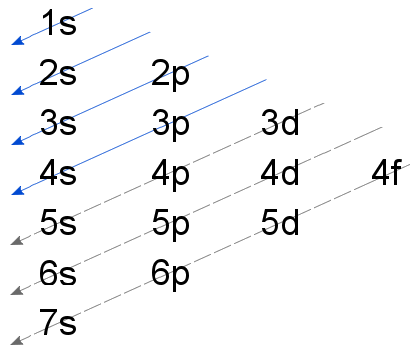
\includegraphics[width=5cm]{src/madelung-rule.png}
\end{figure}
\begin{resume}
    Madelung规则:
    \begin{cenum}
        \item 轨道按$n+l$的大小顺序填充.
        \item 对于相同的$n+l$, 按照$n$上升的次序填充.
    \end{cenum}
\end{resume}

% subsubsection 基态的核外电子排布 (end)

\subsubsection{元素周期律} % (fold)
\label{ssub:元素周期律}

\newpoint{}氢原子的基态电子组态为$\ce{1s}$. 电离能
\[ \abs{E\+_\ce{1s}_} = \abs{-\half m_e c^2 \alpha^2 \rec{1^2}} = \SI{13.6}{\eV}. \]
\newpoint{}氦原子的基态电子组态为$\ce{1s^2}$. 电离能
\[ \abs{E\+_\ce{1s}_} = \abs{-\half m_e c^2 \alpha^2 \frac{Z_{\ce{1s}}^{*2}}{1^2}} = Z_{\ce{1s}}^{*2}\times\SI{13.6}{\eV}. \]
实验值$\SI{24.6}{\eV}$.
\newpoint{}锂元素的基态电子组态为$\ce{1s^2}\ce{2s}$. 电离能
\[ \abs{E\+_\ce{2s}_} = \abs{-\half m_e c^2 \alpha^2 \frac{Z_{\ce{2s}}^{*2}}{1^2}} = Z_{\ce{2s}}^{*2}\times\SI{13.6}{\eV}. \]
实验值$\SI{5.39}{\eV}$.
\newpoint{}锂元素的基态电子组态为$\ce{1s^2}\ce{2s^2}$. 电离能
\[ \abs{E\+_\ce{2s}_} = \abs{-\half m_e c^2 \alpha^2 \frac{Z_{\ce{2s}}^{*2}}{1^2}} = Z_{\ce{2s}}^{*2}\times\SI{13.6}{\eV}. \]
实验值$\SI{9.32}{\eV}$.
\newpoint{}硼元素的基态电子组态为$\ce{1s^2}\ce{2s^2}\ce{2p}$. 电离能
\[ \abs{E\+_\ce{2p}_} = \abs{-\half m_e c^2 \alpha^2 \frac{Z_{\ce{2p}}^{*2}}{1^2}} = Z_{\ce{2p}}^{*2}\times\SI{13.6}{\eV}. \]
实验值$\SI{8.30}{\eV}$. 轨道贯穿减弱, 屏蔽变强.
\newpoint{}碳基态电子组态$\ce{1s^2}\ce{2s^2}\ce{2p^2}$. 电离能$\SI{11.26}{\eV}$.
\newpoint{}氮基态电子组态$\ce{1s^2}\ce{2s^2}\ce{2p^3}$. 电离能$\SI{14.53}{\eV}$.
\newpoint{}氧基态电子组态$\ce{1s^2}\ce{2s^2}\ce{2p^4}$. 电离能$\SI{13.62}{\eV}$. 电离能下降, 原因在于p支壳层中存在反平行的电子, 能级上升.
\newpoint{}氟基态电子组态$\ce{1s^2}\ce{2s^2}\ce{2p^5}$.
\newpoint{}氖基态电子组态$\ce{1s^2}\ce{2s^2}\ce{2p^6}$.
\newpoint{}钠基态电子组态$\ce{1s^2}\ce{2s^2}\ce{2p^6}\ce{3s}$. 电离能$\SI{5.14}{\eV}$.
\newpoint{}镁基态电子组态$\ce{1s^2}\ce{2s^2}\ce{2p^6}\ce{3s^2}$. 电离能$\SI{7.65}{\eV}$.
\newpoint{}第三周期以此类推.
\newpoint{}钾基态电子组态$\ce{[Ar]}\ce{4s}$.
\newpoint{}钙基态电子组态$\ce{[Ar]}\ce{4s^2}$.
\newpoint{}钪基态电子组态$\ce{[Ar]}\ce{3d}\ce{4s^2}$.
\newpoint{}铬基态电子组态$\ce{[Ar]}\ce{3d^{5}}\ce{4s^1}$.
\newpoint{}铜基态电子组态$\ce{[Ar]}\ce{3d^{10}}\ce{4s^1}$.
\newpoint{}锌基态电子组态$\ce{[Ar]}\ce{3d^{10}}\ce{4s^2}$.
\newpoint{}第四周期以此类推.
\newpoint{}铷基态电子组态$\ce{[Kr]}\ce{5s}$.
\newpoint{}锶基态电子组态$\ce{[Kr]}\ce{5s^2}$.
\newpoint{}钇基态电子组态$\ce{[Kr]}\ce{4d^1}\ce{5s^2}$.
\newpoint{}第五周期也存在d和s之间交错的情形.
\newpoint{}第六周期开始$57$号元素开始为镧系元素, 有$\ce{4f}$填充, 之后再填充$\ce{5d}$.
\newpoint{}第七周期开始$89$号元素开始为镧系元素, 有$\ce{5f}$填充, 之后再填充$\ce{6d}$.

% subsubsection 元素周期律 (end)

\subsubsection{电子组态能级} % (fold)
\label{ssub:电子组态能级}

\newpoint{}将各电子能量相加, $\displaystyle \sum E_{n,l}$即为电子组态能级.
\newpoint{}设有$\nu$个电子的电子组态. 如果这$\nu$个电子的$n_i,l_i$均不相同, 则谓之非等效电子组态, 简并度为
\[ G = \prod_{i=1}^\nu 2\pare{2l_i + 1}. \]
\begin{ex}
    氦原子的一个电子被激发到\econfig{3d}, 电子组态为\econfig{1s 3d},
    \[ G = 2\times\pare{2\times 0 + 1}\times 2\times\pare{2\times 2+1} = 20. \]
\end{ex}
处于同一支壳层, 具有相同$n$, $l$值的电子, 谓\gloss{同科电子}.

\paragraph{等效电子组态} % (fold)
\label{par:等效电子组态}

设$\nu$个电子是等效电子, 则该电子组态的简并度为
\[ G = \frac{\brac{2\pare{2l+1}}!}{v!\brac{2\pare{2l+1} - v}!}. \]
\begin{ex}
    氦原子激发到\econfig{1s 2s}, $G = 2\times\pare{2\times 0 + 1}\times 2\times \pare{2\times 0 + 1} = 4$. 基态电子组态\econfig{1s2}对应的
    \[ G = \frac{\brac{2\pare{2\times 0+1}}!}{2!\brac{2\pare{2\times 0+1} - 2}!} = 1. \]
    此时两个电子的$n_1 = n_2 = 1$, $l_1 = l_2 = 0$, $m_{l1} = m_{l2} = 0$, $m_2$必定取$+1/2$和$-1/2$.
\end{ex}

对于满支壳层的电子组态$\nu = 2\pare{2l+1}$, $G=1$, 有
\[ m_l = -l,-l+1,\cdots,l-1,l. \]
而
\[ m_s = \pm\half,\cdots,\pm\half. \]
从而
\[ M\+_L_ = \sum m_l = 0,\quad M\+_S_ = \sum m_s = 0. \]
故$\+vL = \+vS = 0$.

% paragraph 等效电子组态 (end)

% subsubsection 电子组态能级 (end)

\subsubsection{电子组态能级的修正} % (fold)
\label{ssub:电子组态能级的修正}

修正需考虑剩余静电势
\[ \hat H_1 = \sum_{i<j=1}^N \frac{e^2}{4\pi\epsilon_0 r_{ij}} - \sum_{i=1}^n S\pare{r_i}, \]
以及自旋-轨道相互作用
\[ \hat H_2 = \sum_{i=1}^N \xi\pare{r_i} \+vl_i\cdot\+vs_i,\quad \xi\pare{r_i} = \rec{2m_e^2c^2}\rec{r_i}\+d{r_i}d{V\pare{r_i}}. \]

\paragraph{剩余静电势} % (fold)
\label{par:剩余静电势}

由$\displaystyle \sum_{m_i = -l}^{+l} Y_{lm_l}^*\pare{\theta,\phi}Y_{lm_l}\pare{\theta,\phi} = \frac{2l+1}{4\pi}$, 满支壳层组态的电荷分布是球对称的, 只需要计最外层未满支壳层的修正. $H_1$大致与$Z$成正比.

% paragraph 剩余静电势 (end)

\paragraph{自旋-轨道相互作用} % (fold)
\label{par:自旋_轨道相互作用}

满壳层有$\+vL = \+vS = 0$, 故满壳层的自旋-轨道修正为零. 只需考虑最外层未满支壳层的修正. $H_2$大致与$Z^4$成正比.

% paragraph 自旋_轨道相互作用 (end)

\par
对于基态原子或者轻原子的低激发态, 剩余静电势效应更大, 发生$LS$耦合. 在重原子或高激发态的情形, 自旋-轨道相互作用效应更大, 发生$jj$耦合.

% subsubsection 电子组态能级的修正 (end)

%\subsubsection{\titleselect{$LS$耦合情形}{$LS$耦合情形}{LS耦合情形}} % (fold)
\mathsubsubsection{LSCoupling}{$LS$耦合情形}{$LS$耦合情形}{LS耦合情形} % (fold)
\label{ssub:ls耦合情形}

每个电子的轨道角动量不再守恒, 但各轨道角动量耦合成的总轨道角动量$\+vL$是守恒的, $\displaystyle \+vL = \sum_{i=1}^\nu \+vl_i$.
\par
总轨道角动量满足
\[ \+vL^2 = L\pare{L+1}\hbar^2,\quad L_z = M_L \hbar,\quad M_L = -L,-L+1,\cdots,+L. \]
好量子数为
\[ n_1l_1, n_2l_2, \cdots, n_\nu l_\nu,L,M_L. \]
Coulomb能使电子组态能级按不同的$L$分裂. 各电子的不同概率分布造成电子之间不同的Coulomb能.

\par
当自旋平行, Coulomb斥力修正小, 能级低. 当自旋反平行, Coulomb斥力修正大, 能级高. 总自旋角动量满足
\[ \+vS^2 = S\pare{S+1}\hbar^2,\quad S_z = M_s \hbar,\quad M_S = S,S-1,\cdots,-S. \]
$S$是总的角动量量子数, $M_S$是相应的磁量子数. $S$和$M_S$都是好量子数. 交换能使电子组态按$S$的不同而分裂.
\par
在$LS$耦合下, 有$\nu$个价电子的原子用下列量子数描述:
\[ \curb{n_1l_1,n_2l_2,\cdots,n_\nu l_\nu},L,S,M_L,M_S. \]
考虑剩余静电势修正后, 中心力场近似下的电子组态能级简并将部分撤除, 剩余能级按$L$和$S$不同产生分裂.
\begin{ex}
    碳原子的第一激发态\econfig{2p 3p}, 耦合后$L = 2,1,0$, $S = 1,0$. 电子组态能级将按照$L$和$S$的不同组合产生劈裂. $S=1$的三重态能量较低, $S=0$的单重态能量较高.
\end{ex}
由$L,S$决定的能级关于$M_L$和$M_S$仍然是简并的, 简并度为$\pare{2L+1}\pare{2S+1}$. 原子光谱学中将这简并的$\pare{2L+1}\pare{2S+1}$个态称为原子的多重态或多重项, 记作$^{2S+1}L$. 其中$L=0,1,2,3,\cdot$分别用S, P, D, F标记.

\begin{center}
    \begin{tabular}{cc}
        & $\ce{^1S}$ \\
        & $\ce{^1P}$ \\
        & $\ce{^1D}$ \\
        \econfig{2p3p} $\mapsto$ & \\
        & $\ce{^3S}$ \\
        & $\ce{^3P}$ \\
        & $\ce{^3D}$
    \end{tabular}
\end{center}

$\+vJ$满足
\[ \+vJ^2 = J\pare{J+1}\hbar^2,\quad J = L+S,\cdots,\abs{L-S}. \]
且
\[ J_z = J,J-1,\cdots,-J. \]
此时系统由如下量子数描述:
\[ \curb{n_1l_1,n_2l_2,\cdots,n_\nu l_\nu},L,S,J,M_J. \]
此时再考虑精细结构修正, 多重态能级的$\pare{2L+1}\pare{2S+1}$重简并撤除, 能级按照$J$产生分裂. 用${^{2S+1}L_J}$表示\gloss{子项}.
\par
精细结构修正为
\[ \Delta E_J = \frac{\hbar^2}{2}\xi\pare{L,S} \brac{J\pare{J+1} - L\pare{L+1} - S\pare{S+1}}. \]
同一多重态相邻能级的间隔为
\[ E_J = E_{J-1} = \frac{\hbar^2}{2}\xi\pare{L,S}\pare{J\pare{J+1} - \pare{J-1}J}  = \xi\pare{L,S}\hbar^2 J. \]
\begin{cenum}
    \item $\xi\pare{L,S} > 0$: 同一多重态能级中, $J$越小, 能量越低, 谓\gloss{正常次序的多重态}.
    \item $\xi\pare{L,S} < 0$: 同一多重态能级中, $J$越大, 能量越低, 谓\gloss[2em]{倒转次序的多重态}.
    \item 典型的$LS$耦合下, $\resumath{\text{$J$和$J-1$的能级差大体和$J$成正比.}}$
\end{cenum}
非等效电子组态, 如碳原子的第一激发态 \econfig{2p 3p} 状态数目为
\[ G\pare{\text{\econfig{2p 3p}}} = 36. \]
在$LS$耦合下分属多重态
\[ \ce{^3D_{1,2,3}},\ce{^3P_{0,1,2}},\ce{^3S_{1}},\ce{^1D_2},\ce{^1P_1},\ce{^1S_0}. \]
而基态 \econfig{2p2} 的状态数目为$\displaystyle C_6^2 = 15$.
\par
用$m_{l_1}^{m_{s1}}m_{l_2}^{m_{s2}}$表示两个电子的态, 对于 \econfig{2p 3p} 可以列出
\[ \begin{array}{c|ccc}
    &   & M_S & \\
    \hline
    & 1 & 2   & 1\\
    & 2 & 4   & 2\\
M_L & 3 & 6   & 3\\
    & 2 & 4   & 2\\
    & 1 & 2   & 1
\end{array}. \]
对于 \econfig{2p2} 可以列出
\[ \begin{array}{c|ccc}
    &   & M_S & \\
    \hline
    &   & 1   & \\
    & 1 & 2   & 1\\
M_L & 1 & 3   & 1\\
    & 1 & 2   & 1\\
    &   & 1   &
\end{array}. \]
\begin{pitfall}
    计重数时应考虑电子之不可区分性.
\end{pitfall}
可以分解为(\gloss{Slater作图法})
\[ \begin{array}{c|ccc}
    &   & M_S & \\
    \hline
    &   & 1   & \\
    & 1 & 2   & 1\\
M_L & 1 & 3   & 1\\
    & 1 & 2   & 1\\
    &   & 1   &
\end{array} = \underbrace{\begin{array}{c|ccc}
    &   & M_S & \\
    \hline
    &   & 1   & \\
    &   & 1   & \\
M_L &   & 1   & \\
    &   & 1   & \\
    &   & 1   &
\end{array}}_{\ce{^1D}} + \underbrace{\begin{array}{c|ccc}
    &   & M_S & \\
    \hline
    &   &     & \\
    & 1 & 1   & 1 \\
M_L & 1 & 1   & 1 \\
    & 1 & 1   & 1 \\
    &   &     &
\end{array}}_{\ce{^3P}} + \underbrace{\begin{array}{c|ccc}
    &   & M_S & \\
    \hline
    &   &     & \\
    &   &     &   \\
M_L &   & 1   &   \\
    &   &     &   \\
    &   &     &
\end{array}}_{\ce{^1S}}. \]
对于两个电子的情形, 有更简单的法则, $\resumath{\text{$L+S$必定为偶数}.}$ 空间波函数的宇称为$\pare{-1}^L$. 当$L$为偶数, 空间波函数对称, 自旋波函数反对称, $S=0$. 当$L$为奇数, 同理有$S=1$.
\begin{ex}
    对于$n\mathrm{d}^2$, $l_1 = l_2 = 2$, $L = 0,1,2,3,4$, $s_1 = s_2 = 1/2$, $S=0,1$,
    \begin{cenum}
        \item $S=0$, $L=0,2,4$, $\Rightarrow \ce{^1G_4}$, $\ce{^1D_2}$, $\ce{^1S_0}$.
        \item $S=1$, $L=1,3$, $\Rightarrow \ce{^3P_{2,1,0}}, \ce{^3F_{4,3,2}}$.
    \end{cenum}
\end{ex}
考虑等效电子组态$\pare{nl}^\nu$和$\pare{nl}^{Y-\nu}$, 对于满支壳层电子组态$\pare{nl}^Y$, $L=S=0$. 故
\[ \pare{M_L}_\nu + \pare{M_L}_{Y-\nu} = 0. \]
即
\[ \pare{M_L}_\nu = -\pare{M_L}_{Y-\nu} \Rightarrow \pare{L}_\nu = \pare{L}_{Y-\nu},\quad \pare{S}_\nu = \pare{S}_{Y-\nu}. \]
互补电子组态具有相同个原子态谱项.
\begin{ex}
    氟原子的激发态电子组态为 \econfig{2p4 3s}, 求它在$LS$耦合下可能的原子态. 先求 \econfig{2p4} 谱项, 即 \econfig{2p2}的互补组态, 具有相同的谱项
        \[ \ce{^3P}, \ce{^1D}, \ce{^1S}. \]
        再和 \econfig{3s} 耦合.
    \begin{cenum}
        \item $\ce{^3P}$: $L'=1$, $l=0$, $\Rightarrow L=1$. $S'=1$, $s=1/2$, $\Rightarrow S=3/2,1/2$. 合成为$\ce{^4P_{5/2,3/2,1/2}}$和$\ce{^2P_{3/2,1/2}}$.
        \item $\ce{^1D}$: 合成为$\ce{^2D_{5/2,3/2}}$.
        \item $\ce{^1S}$: 合成为$\ce{^2S_{1/2}}$.
    \end{cenum}
\end{ex}

% subsubsection ls耦合情形 (end)

\mathsubsubsection{jjcase}{$jj$耦合情形}{$jj$耦合情形}{jj耦合情形} % (fold)
\label{ssub:jj耦合情形}

若自旋-轨道相互作用远大于剩余静电势, $\hat H_2 \gg \hat H_1$, 则应先考虑自旋-轨道相互作用引起的电子组态能级分裂. 电子视为各自独立地在中心场中运动. $\nu$个价电子的组态为
\[ n_1l_1,n_2l_2,\cdots,n_\nu l_\nu. \]
相应的
\[ \hat H_2 = \sum_{i=1}^\nu \xi\pare{r_i} \+vl_i\cdot \+vs_i. \]
每个电子的$\+vl$和$\+vs$耦合成单个电子的总角动量$\+vj$,
\[ \+vj = \+vl + \+vs. \]
单电子的量子数由$\pare{n,l,m_l,m_s}$变为$\pare{n,l,j,m_j}$描述. 在$jj$耦合下有$\nu$个价电子的量子态由
\[ \pare{n_1,l_1,j_1,m_{j1}},\cdots,\pare{n_\nu,l_\nu,j_\nu,m_{j\nu}}. \]
单个电子的自旋-轨道修正为
\[ \Delta E_{nlj} = \frac{\hbar^2}{2}\xi\pare{n,l}\brac{j\pare{j+1} - l\pare{l+1} - s\pare{s+1}}. \]
总修正为
\[ \Delta E = \sum E_{nlj}. \]
中心力场近似下电子组态能级的简并部分撤除, 能级按照价电子$j_i$的不同组合产生分裂, 其中最小的$j_i$组合的能级最低.
\par
对于$\nu$个电子的组态, 用$\pare{j_1,\cdots,j_\nu}$表示$jj$耦合下的原子多重态.
\begin{ex}
    考虑$n\mathrm{s}\,n'\mathrm{p}$电子组态能级在$jj$耦合下的劈裂, 两个电子分别为
    \[ l_1 = 0,\quad s_1=\half,\quad j_1=\half \]
    和
    \[ l_2 = 1,\quad s_2=\half,\quad j_2=\frac{3}{2},\half. \]
    分裂为两个多重态能级.
\end{ex}
此时再进一步考虑剩余静电势的修正, 单粒子的$\+vj$不再守恒, $m_j$不再是好量子数. 引入总角动量
\[ \+vJ = \sum_{i=1}^\nu \+vj_i, \]
多重态的能级简并进一步撤除, 能级按照$J$的不同产生分裂. 相应的精细结构子项表示为
\[ \pare{j_1,j_2,\cdot,j_\nu}_J. \]
\begin{ex}
    对于多重态$\displaystyle \pare{\half,\frac{3}{2}}$, $\displaystyle j_1 = \half, j_2 = \frac{3}{2} \Rightarrow J = 2,1$. 分裂为两条. 对于多重态$\displaystyle \pare{\half,\half}$, $\displaystyle j_1 = \half, j_2 = \frac{3}{2} \Rightarrow J = 1,0$. 分裂为两条.
    \begin{center}
        \begin{tabular}{ccc}
            \+:r5{$n\mathrm{s}n'\mathrm{p}$} & \+:r2{$\pare{1/2,3/2}$} & $\pare{1/2,3/2}_1$ \\
             &  & $\pare{1/2,3/2}_0$ \\
             \\
            & \+:r2{$\pare{1/2,1/2}$} & $\pare{1/2,1/2}_1$ \\
             &  & $\pare{1/2,1/2}_0$ \\
            $\hat H_0$ & $\hat H_2$ & $\hat H_1$
        \end{tabular}
    \end{center}
\end{ex}
\begin{remark}
    对于基态原子和轻原子的低激发态, 采用$LS$耦合. 对于重原子或高激发态, 采用$jj$耦合.
\end{remark}
\begin{ex}
    碳和硅的低激发态为典型的$LS$耦合($^1\mathrm{P}_1$和$^3\mathrm{P}_{2,1,0}$), 硒和铅的低激发态为典型的$jj$耦合. 锗位于二者之间.
\end{ex}

% subsubsection jj耦合情形 (end)

\mathsubsubsection{comparison}{两者比较}{$LS$耦合与$jj$耦合比较}{LS耦合与jj耦合比较} % (fold)
\label{ssub:ls耦合与jj耦合比较}

\begin{ex}
    考虑硅的${3\mathrm{p}\,n\mathrm{s}}$能级. 当两个电子中的一个进入高激发态时, 两个电子之间的静电相互作用迅速减小, 静电非中心力也迅速减小.
\end{ex}

% subsubsection ls耦合与jj耦合比较 (end)

\subsubsection{Hund规则和原子基态} % (fold)
\label{ssub:hund规则和原子基态}

基态一般遵守$LS$耦合, 能级会发生分裂, 其中真正的基态满足\gloss{Hund规则}.
\begin{resume}
    \begin{cenum}
        \item 对于一给定的电子组态, 能量最低的原子态必定具有Pauli原理所允许的最大$S$值.
        \item $S$相同的状态中, $L$值最大的能量最低.
        \item 对于等效电子组态$\pare{nl}^\nu$,
        \begin{cenum}
            \item 当$\nu<{2l+1}$, 即未达到半满时, 多重态中$J$值最小的状态能量最低, 谓\gloss{正常次序}.
            \item 当$\nu>{2l+1}$, 即超过半满时, 多重态中$J$值最大的能量最低, 谓\gloss{倒转次序}.
        \end{cenum}
    \end{cenum}
\end{resume}
\begin{ex}
    满支壳层的电子组态$\+vL=\+vS=0$, 例如惰性气体, 基态只能为$^1\mathrm{S}_0$.
\end{ex}
\begin{ex}
    对于氮原子($\mathrm{p}$恰好半满),
    \begin{cenum}
        \item $S$最大的能量最低, 故三个自旋平行, $\displaystyle M_S = \frac{3}{2}$.
        \item $L$最大的能量最低, $m_l$只能取$\pare{+1,0,-1}$, $L=0$.
    \end{cenum}
\end{ex}
\begin{ex}
    对于碳原子($2\mathrm{p}^2$小于半满),
    \begin{cenum}
        \item $S$最大的能量最低, 故两个自旋平行, $\displaystyle M_S = 1$.
        \item $L$最大的能量最低, $m_l$只能取$\curb{+1,0}$, $L=1$, $J=\curb{0,1,2}$.
        \item 正常次序, $J$值最小的能量最低, 故基态为$^3\mathrm{P}_0$.
    \end{cenum}
\end{ex}
\begin{ex}
    对于氧原子($2\mathrm{p}^4$大于半满), 前两条法则同$^2\mathrm{P}_2$,
    \begin{cenum}
        \item $S$最大的能量最低, 故自旋为$\pare{\uparrow\downarrow}\pare{\uparrow}\pare{\uparrow}$, $\displaystyle M_S = 1$.
        \item $L$最大的能量最低, $L=1$, $J=\curb{0,1,2}$.
        \item 倒转次序, $J$值最大的能量最低, 故基态为$^3\mathrm{P}_2$.
    \end{cenum}
\end{ex}

% subsubsection hund规则和原子基态 (end)

\subsubsection{外磁场中多重态的能级分裂} % (fold)
\label{ssub:外磁场中多重态的能级分裂}

弱磁场的情形下, 原子磁矩和外磁场的作用弱, 不破坏$LS$耦合和$jj$耦合. 原子总有效磁矩与磁场作用, 取向势能为
\[ U = -\+v\mu_J\cdot \+vB. \]
多电子原子的有效磁矩
\[ \+v\mu_J = -g_J \frac{\mu\+_B_}{\hbar}\+vJ. \]
$g_J$是多电子原子的Land\'e因子, 对于$LS$耦合为
\[ \resumath{g_J = 1 + \frac{J\pare{J+1} + S\pare{S+1} - L\pare{L+1}}{2J\pare{J+1}}.} \]
外磁场引起的能量变化为
\[ \Delta E = M_J g_J\mu\+_B_B. \]

% subsubsection 外磁场中多重态的能级分裂 (end)

\subsubsection{电偶极跃迁的选择定则} % (fold)
\label{ssub:电偶极跃迁的选择定则}

跃迁速率为
\[ \lambda_{fi} = \frac{\omega^3}{6\epsilon_0 hc^3}\abs{\expc{\+vp}}^2 = \frac{\omega^3}{6\epsilon_0 hc^3}\abs{\int u_f^* \pare{-e\+vr}u_i\,\rd{\tau}}^2 \neq 0. \]
\gloss{Laporte定则}表明\hl{跃迁只允许在宇称相反的态之间发生}. 中心力场下, 单电子的波函数为
\[ u_{nlm_l}\pare{\+vr} = R_{nl}\pare{r}Y_{lm_l}\pare{\theta,\phi}. \]
在空间反演$\+vr\mapsto -\+vr$下, 变为
\[ Y_{lm_l}\pare{\pi-\theta,\pi+\phi} = \pare{-1}^l Y_{lm_l}\pare{\theta,\phi}. \]
如果$l$为偶数, 则状态具有偶宇称. 若$l$为奇数, 则谓之具有奇宇称. 对于多电子原子, 在中心力场近似下, 宇称为$\pare{-1}^{l_1+\cdots+l_\nu}$. 电偶极辐射中, 光子带走的角动量为$\hbar$, 要求电偶极跃迁的选择定则为
\[ \Delta \sum l_i = \pm 1. \]
一般情形下, 原子光谱只涉及单电子的跃迁, 此时选择定则简化为
\[ \resumath{\Delta l = \pm 1.} \]
\begin{resume}
$LS$耦合的选择定则为
\[ \begin{cases}
    \Delta S = 0, \\
    \Delta L = 0, \pm 1, \\
    \Delta J = 0, \pm 1, & J=0\mapsto J=0\text{除外} \\
    \Delta M_J = 0, \pm 1, & \Delta J =0, J=0\mapsto J=0\text{除外}.
\end{cases} \]
$jj$耦合的选择定则为
\[ \begin{cases}
    \Delta j = 0,\pm 1,\\
    \Delta J = 0,\pm 1, & J=0\mapsto J=0\text{除外}, \\
    \Delta M_J = 0,\pm 1, & \Delta J =0, J=0\mapsto J=0\text{除外}.
\end{cases} \]
\end{resume}
\begin{ex}
    钠原子的$\ce{3s}$可激发到$n\mathrm{l}$. 各个态对应的谱项为
    \[ \mathrm{s}: ^2\mathrm{S}_{1/2},\quad \mathrm{p}: ^2\mathrm{P}_{1/2,3/2},\quad \mathrm{D}: ^2\mathrm{D}_{3/2,5/2},\quad \mathrm{F}: ^2\mathrm{F}_{5/2,7/2}. \]
    由电偶极跃迁的选择定则
    \[ \Delta = \pm 1,\quad \Delta j = 0,\pm 1 \]
    可得各谱线.
\end{ex}

% subsubsection 电偶极跃迁的选择定则 (end)

% subsection 多电子原子 (end)

\subsection{原子内层能级和特征X射线} % (fold)
\label{sub:原子内层能级和特征x射线}

\subsubsection{X射线的能谱} % (fold)
\label{ssub:x射线的能谱}

高能电子束射入金属, 可得连续的韧致辐射谱和离散的X射线谱. 连续谱满足
\[ h\nu\+_max_ = \frac{hc}{\lambda\+_min_} = eU. \]
当电压大于一定值, 连续谱上将出现一定的分立谱. 其波长与加速电压无关, 仅与靶材料有关. 不同靶材料除了波长不同, X射线谱具有相似的结构.
\par
特征谱包括两组谱线,
\[ \begin{cases}
    \text{$\mathrm K$线系:} & \mathrm K_\alpha, \mathrm K_\beta, \mathrm K_\gamma, \cdots, \\
    \text{$\mathrm L$线系:} & \mathrm L_\alpha, \mathrm L_\beta, \mathrm L_\gamma, \cdots.
\end{cases} \]
原子序数大的元素还会出现$\mathrm M$线, $\mathrm N$线等. \gloss{Moseley公式}表明
\[ \begin{cases}
    \mathrm K_\alpha: & \displaystyle \tilde{\nu}\+_K_ = R\pare{Z-1}^2\pare{\rec{1^2} - \rec{2^2}}, \\[.5em]
    \mathrm L_\alpha: & \displaystyle \tilde{\nu}\+_K_ = R\pare{Z-7.4}^2\pare{\rec{2^2} - \rec{3^2}}.
\end{cases} \]
根据实验测量的特征线波数, 在Moseley图上就可以标识元素的种类, 所以特征谱又谓标识谱. 为了让$2\mapsto 1$的跃迁发生, 需要在$\mathrm K$层制造空穴, 这要求使用高能电子电离之.
\par
例如镉的最外层为 \econfig{5s2 4d10}, 各层皆填满, 基态$^1\mathrm S_0$. 可以激发到 \econfig{5s5p}, \econfig{5s 6p}, \econfig{5s 7p} 等. 也可以激发到 \econfig{5s 6s}, \econfig{5s 7s} 等.
\par
当$\mathrm K$壳层电离一个电子后, 相应的基态变为$^2\mathrm S_{1/2}$, 此时能级最高. $\mathrm L$壳层电离一个$2\mathrm{s}$电子后相应的基态也变为$^2\mathrm S_{1/2}$. 电离$2\mathrm p$电子则基态变为$^2\mathrm P_{1/2,3/2}$, 从而$\mathrm L$壳层的电离有三支. $\mathrm M$壳层电离一个$3\mathrm{s}$电子后相应的基态也变为$^2\mathrm S_{1/2}$. 电离$3\mathrm p$电子则基态变为$^2\mathrm P_{1/2,3/2}$, 电离$3d$电子则基态变为$^2\mathrm D_{3/2,5/2}$, 从而$M$壳层的电离有五支.
\par
以$\mathrm K$, $\mathrm L\+_I_$, $\mathrm L\+_II_$, $\mathrm L\+_III_$等表示相应壳层电离一个电子后的能级. 则$\mathrm K\mapsto \mathrm L\+_II,III_$是允许的跃迁, $\mathrm K\mapsto \mathrm M\+_II, III_$也是允许的跃迁, 还可以跃迁到$N$能级. 分别为$\mathrm K_\alpha$和$\mathrm K_\beta$线系.
\begin{center}
    \begin{tikzpicture}
        \draw[dashed] (0,0) node[left] {$\mathrm{N}$} -- (8,0) node[right] {};
        \draw (0,2) node[left] {$\mathrm{M}\+_V_$} -- (8,2) node[right] {$^2\mathrm D_{5/2}$};
        \draw (0,2.5) node[left] {$\mathrm{M}\+_IV_$} -- (8,2.5) node[right] {$^2\mathrm D_{3/2}$};
        \draw (0,3.5) node[left] {$\mathrm{M}\+_III_$} -- (8,3.5) node[right] {$^2\mathrm P_{3/2}$};
        \draw (0,4) node[left] {$\mathrm{M}\+_II_$} -- (8,4) node[right] {$^2\mathrm P_{1/2}$};
        \draw (0,5) node[left] {$\mathrm{M}\+_I_$} -- (8,5) node[right] {$^2\mathrm S_{1/2}$};
        \draw (0,7) node[left] {$\mathrm{L}\+_III_$} -- (8,7) node[right] {$^2\mathrm P_{3/2}$};
        \draw (0,7.5) node[left] {$\mathrm{L}\+_II_$} -- (8,7.5) node[right] {$^2\mathrm P_{1/2}$};
        \draw (0,8.5) node[left] {$\mathrm{L}\+_I_$} -- (8,8.5) node[right] {$^2\mathrm S_{1/2}$};
        \draw (0,10.5) node[left] {$\mathrm{K}$} -- (8,10.5) node[right] {$^2\mathrm S_{1/2}$};
        \draw[latex-latex] (1,10.5) -- (1,7.5) node[midway,fill=white] {$\alpha_2$};
        \draw[latex-latex] (1.5,10.5) -- (1.5,7) node[midway,fill=white] {$\alpha_1$};
        \draw[latex-latex] (2,10.5) -- (2,4) node[midway,fill=white] {$\beta_1$};
        \draw[latex-latex] (2.5,10.5) -- (2.5,3.5) node[midway,fill=white] {$\beta_3$};
        \draw[latex-latex] (3,10.5) -- (3,0) node[midway,fill=white] {$\beta_{\cdots}$};
        \draw[latex-latex] (3.5,8.5) -- (3.5,4) node[midway,fill=white] {$\beta_{4}$};
        \draw[latex-latex] (4,8.5) -- (4,3.5) node[midway,fill=white] {$\beta_{3}$};
        \draw[latex-latex] (4.5,7.5) -- (4.5,5) node[midway,fill=white] {$\eta$};
        \draw[latex-latex] (5,7.5) -- (5,2.5) node[midway,fill=white] {$\beta_1$};
        \draw[latex-latex] (5.5,7) -- (5.5,5) node[midway,fill=white] {$l$};
        \draw[latex-latex] (6,7) -- (6,2.5) node[midway,fill=white] {$\alpha_2$};
        \draw[latex-latex] (6.5,7) -- (6.5,2) node[midway,fill=white] {$\alpha_1$};
        \draw[latex-latex] (7,7) -- (7,0) node[midway,fill=white] {$\beta_2$};
    \end{tikzpicture}
\end{center}

% subsubsection x射线的能谱 (end)

\subsubsection{Auger电子能谱} % (fold)
\label{ssub:auger电子能谱}

$\mathrm K$壳层出现空穴后, $\mathrm L$壳层上的一个$\mathrm s$电子可能跃迁到$\mathrm K$壳层填补这一空位, 释放出的能量导致一个$\mathrm 2p$电子电离, 谓$\mathrm K\mathrm L\+_I_\mathrm L\+_II,III_$跃迁. 其动能
\[ E\+_A_ = E\+_K_ - E\+_{L\+_I_}_ - E\+_{L\+_II,III_}_. \]
X荧光发射和Auger发射是随机的.

% subsubsection auger电子能谱 (end)

\subsubsection{荧光产额} % (fold)
\label{ssub:荧光产额}

荧光产额为
\[ \omega\+_K_ = \frac{K\text{X光子数}}{\text{有$K$层空位的原子数}}, \]
有
\[ \omega\+_K_ \approx \pare{1+b_K Z^4}^{-1},\quad b_K \approx 7.5\times 10^{-5}. \]
重元素的$\mathrm K$层以荧光过程为主, 氢元素以Auger过程为主.

% subsubsection 荧光产额 (end)

% subsection 原子内层能级和特征x射线 (end)

% section 多电子原子 (end)

\end{document}
